% Options for packages loaded elsewhere
% Options for packages loaded elsewhere
\PassOptionsToPackage{unicode}{hyperref}
\PassOptionsToPackage{hyphens}{url}
%
\documentclass[
  ignorenonframetext,
  aspectratio=169,
  russian,
  aspectratio=169]{beamer}
\newif\ifbibliography
\usepackage{pgfpages}
\setbeamertemplate{caption}[numbered]
\setbeamertemplate{caption label separator}{: }
\setbeamercolor{caption name}{fg=normal text.fg}
\beamertemplatenavigationsymbolshorizontal
% remove section numbering
\setbeamertemplate{part page}{
  \centering
  \begin{beamercolorbox}[sep=16pt,center]{part title}
    \usebeamerfont{part title}\insertpart\par
  \end{beamercolorbox}
}
\setbeamertemplate{section page}{
  \centering
  \begin{beamercolorbox}[sep=12pt,center]{section title}
    \usebeamerfont{section title}\insertsection\par
  \end{beamercolorbox}
}
\setbeamertemplate{subsection page}{
  \centering
  \begin{beamercolorbox}[sep=8pt,center]{subsection title}
    \usebeamerfont{subsection title}\insertsubsection\par
  \end{beamercolorbox}
}
% Prevent slide breaks in the middle of a paragraph
\widowpenalties 1 10000
\raggedbottom
\AtBeginPart{
  \frame{\partpage}
}
\AtBeginSection{
  \ifbibliography
  \else
    \frame{\sectionpage}
  \fi
}
\AtBeginSubsection{
  \frame{\subsectionpage}
}
\usepackage{iftex}
\ifPDFTeX
  \usepackage[T1]{fontenc}
  \usepackage[utf8]{inputenc}
  \usepackage{textcomp} % provide euro and other symbols
\else % if luatex or xetex
  \usepackage{unicode-math} % this also loads fontspec
  \defaultfontfeatures{Scale=MatchLowercase}
  \defaultfontfeatures[\rmfamily]{Ligatures=TeX,Scale=1}
\fi
\usepackage{lmodern}

\usefonttheme{serif} % use mainfont rather than sansfont for slide text
\ifPDFTeX\else
  % xetex/luatex font selection
  \setmainfont[]{DejaVu Serif}
  \setsansfont[]{DejaVu Sans}
  \setmonofont[]{DejaVu Sans Mono}
\fi
% Use upquote if available, for straight quotes in verbatim environments
\IfFileExists{upquote.sty}{\usepackage{upquote}}{}
\IfFileExists{microtype.sty}{% use microtype if available
  \usepackage[]{microtype}
  \UseMicrotypeSet[protrusion]{basicmath} % disable protrusion for tt fonts
}{}


\usepackage{longtable,booktabs,array}
\newcounter{none} % for unnumbered tables
\usepackage{calc} % for calculating minipage widths
\usepackage{caption}
% Make caption package work with longtable
\makeatletter
\def\fnum@table{\tablename~\thetable}
\makeatother
\usepackage{graphicx}
\makeatletter
\newsavebox\pandoc@box
\newcommand*\pandocbounded[1]{% scales image to fit in text height/width
  \sbox\pandoc@box{#1}%
  \Gscale@div\@tempa{\textheight}{\dimexpr\ht\pandoc@box+\dp\pandoc@box\relax}%
  \Gscale@div\@tempb{\linewidth}{\wd\pandoc@box}%
  \ifdim\@tempb\p@<\@tempa\p@\let\@tempa\@tempb\fi% select the smaller of both
  \ifdim\@tempa\p@<\p@\scalebox{\@tempa}{\usebox\pandoc@box}%
  \else\usebox{\pandoc@box}%
  \fi%
}
% Set default figure placement to htbp
\def\fps@figure{htbp}
\makeatother



\ifLuaTeX
\usepackage[bidi=basic,shorthands=off,provide=*]{babel}
\else
\usepackage[bidi=default,shorthands=off,provide=*]{babel}
\fi
\ifPDFTeX
\else
\babelfont{rm}[]{DejaVu Serif}
\fi
\ifLuaTeX
  \usepackage{selnolig} % disable illegal ligatures
\fi


\setlength{\emergencystretch}{3em} % prevent overfull lines

\providecommand{\tightlist}{%
  \setlength{\itemsep}{0pt}\setlength{\parskip}{0pt}}



 

\usepackage[]{csquotes}

\IfFileExists{plex-otf.sty}{
  %% Full TeXlive
  % \usepackage[%
  %   % math,
  %   RM={Scale=0.94},SS={Scale=0.94},SScon={Scale=0.94},TT={Scale=MatchLowercase,FakeStretch=0.9},DefaultFeatures={Ligatures=Common}
  % ]{plex-otf}
}{
  %% TinyTeX
  \usepackage{libertine}
}

%%% Load theme
% https://deic.uab.cat/~iblanes/beamer_gallery/
\IfFileExists{beamerthemegotham.sty}{
  %% Full TeXlive
  \usetheme{gotham}
  \gothamset{
    numbering=totalpagenumber,
    parttocframe default=off,
    sectiontocframe default=off,
    subsectiontocframe default=off,
  }
}{
  %% TinyTeX
  \usetheme{Madrid}
}
\makeatletter
\@ifpackageloaded{caption}{}{\usepackage{caption}}
\AtBeginDocument{%
\ifdefined\contentsname
  \renewcommand*\contentsname{Содержание}
\else
  \newcommand\contentsname{Содержание}
\fi
\ifdefined\listfigurename
  \renewcommand*\listfigurename{Список иллюстраций}
\else
  \newcommand\listfigurename{Список иллюстраций}
\fi
\ifdefined\listtablename
  \renewcommand*\listtablename{Список таблиц}
\else
  \newcommand\listtablename{Список таблиц}
\fi
\ifdefined\figurename
  \renewcommand*\figurename{Рисунок}
\else
  \newcommand\figurename{Рисунок}
\fi
\ifdefined\tablename
  \renewcommand*\tablename{Таблица}
\else
  \newcommand\tablename{Таблица}
\fi
}
\@ifpackageloaded{float}{}{\usepackage{float}}
\floatstyle{ruled}
\@ifundefined{c@chapter}{\newfloat{codelisting}{h}{lop}}{\newfloat{codelisting}{h}{lop}[chapter]}
\floatname{codelisting}{Список}
\newcommand*\listoflistings{\listof{codelisting}{Листинги}}
\makeatother
\makeatletter
\makeatother
\makeatletter
\@ifpackageloaded{caption}{}{\usepackage{caption}}
\@ifpackageloaded{subcaption}{}{\usepackage{subcaption}}
\makeatother

\usepackage{bookmark}
\IfFileExists{xurl.sty}{\usepackage{xurl}}{} % add URL line breaks if available
\urlstyle{same}
\hypersetup{
  pdftitle={Выполнение лабораторной работы №8},
  pdfauthor={Карпухин Клим},
  pdflang={ru-RU},
  hidelinks,
  pdfcreator={LaTeX via pandoc}}


\title{\texorpdfstring{Выполнение лабораторной работы
№8}{Выполнение лабораторной работы №8}}
\subtitle{\texorpdfstring{Анализ файловой системы Linux. Команды для
работы с файлами и
каталогами.}{Анализ файловой системы Linux. Команды для работы с файлами и каталогами.}}
\author{Карпухин Клим}
\date{2026-03-28}

\begin{document}
\frame{\titlepage}


\section{Информация о
докладчике}\label{ux438ux43dux444ux43eux440ux43cux430ux446ux438ux44f-ux43e-ux434ux43eux43aux43bux430ux434ux447ux438ux43aux435}

\begin{frame}{Докладчик}
\protect\phantomsection\label{ux434ux43eux43aux43bux430ux434ux447ux438ux43a}
\begin{columns}[c]
\begin{column}{0.65\linewidth}
\begin{itemize}[<+->]
\tightlist
\item
  \textbf{Карпухин Клим}
\item
  Российский университет дружбы народов
\item
  Email:
  \href{mailto:1032255580@rudn.ru}{\nolinkurl{1032255580@rudn.ru}}
\item
  Роль: студент (лабораторная работа по ОС/виртуализации)
\end{itemize}
\end{column}
\end{columns}
\end{frame}

\section{Вводная
часть}\label{ux432ux432ux43eux434ux43dux430ux44f-ux447ux430ux441ux442ux44c}

\begin{frame}[fragile]{Актуальность}
\protect\phantomsection\label{ux430ux43aux442ux443ux430ux43bux44cux43dux43eux441ux442ux44c}
\begin{itemize}[<+->]
\tightlist
\item
  Файловая система Linux --- основа любой Unix-подобной системы.
\item
  Умение управлять файлами и каталогами через командную строку
  необходимо для администрирования, разработки и повседневной работы.
\item
  Знание команд \texttt{cp}, \texttt{mv}, \texttt{chmod},
  \texttt{mount}, \texttt{df}, \texttt{fsck} позволяет эффективно
  работать с дисками, правами доступа и структурой каталогов.
\item
  Лабораторная работа даёт практические навыки, которые пригодятся в
  дальнейшем изучении операционных систем.
\end{itemize}
\end{frame}

\begin{frame}{Объект и предмет исследования}
\protect\phantomsection\label{ux43eux431ux44aux435ux43aux442-ux438-ux43fux440ux435ux434ux43cux435ux442-ux438ux441ux441ux43bux435ux434ux43eux432ux430ux43dux438ux44f}
\begin{itemize}[<+->]
\tightlist
\item
  \textbf{Объект:} файловая система Linux и способы управления ею.
\item
  \textbf{Предмет:} команды для копирования, перемещения, изменения прав
  доступа, а также утилиты для анализа и обслуживания файловой системы.
\end{itemize}
\end{frame}

\section{Научная новизна и практическая
значимость}\label{ux43dux430ux443ux447ux43dux430ux44f-ux43dux43eux432ux438ux437ux43dux430-ux438-ux43fux440ux430ux43aux442ux438ux447ux435ux441ux43aux430ux44f-ux437ux43dux430ux447ux438ux43cux43eux441ux442ux44c}

\begin{frame}[fragile]{Научная новизна}
\protect\phantomsection\label{ux43dux430ux443ux447ux43dux430ux44f-ux43dux43eux432ux438ux437ux43dux430}
\begin{itemize}[<+->]
\tightlist
\item
  Изучение поведения стандартных команд Unix/Linux в реальной среде
  Fedora Sway.
\item
  Демонстрация влияния прав доступа на возможность чтения, записи и
  выполнения файлов и каталогов.
\item
  Практическое знакомство с утилитами \texttt{mount}, \texttt{df},
  \texttt{fsck}, \texttt{mkfs} через справочную систему \texttt{man}.
\end{itemize}
\end{frame}

\begin{frame}[fragile]{Практическая значимость работы}
\protect\phantomsection\label{ux43fux440ux430ux43aux442ux438ux447ux435ux441ux43aux430ux44f-ux437ux43dux430ux447ux438ux43cux43eux441ux442ux44c-ux440ux430ux431ux43eux442ux44b}
\begin{itemize}[<+->]
\tightlist
\item
  Полученные навыки позволяют уверенно копировать, перемещать и
  переименовывать файлы и каталоги.
\item
  Освоение \texttt{chmod} даёт возможность гибко управлять доступом к
  объектам.
\item
  Умение анализировать состояние файловой системы (\texttt{mount},
  \texttt{df}) полезно для диагностики и оптимизации работы системы.
\item
  Понимание утилит \texttt{fsck}, \texttt{mkfs}, \texttt{kill} расширяет
  кругозор в системном администрировании.
\end{itemize}
\end{frame}

\section{Цель, гипотеза и
задачи}\label{ux446ux435ux43bux44c-ux433ux438ux43fux43eux442ux435ux437ux430-ux438-ux437ux430ux434ux430ux447ux438}

\begin{frame}{Цель}
\protect\phantomsection\label{ux446ux435ux43bux44c}
Ознакомиться с файловой системой Linux, её структурой, именами и
содержанием каталогов, а также приобрести практические навыки применения
команд для работы с файлами и каталогами, управления процессами и
обслуживания файловой системы.
\end{frame}

\begin{frame}[fragile]{Гипотеза}
\protect\phantomsection\label{ux433ux438ux43fux43eux442ux435ux437ux430}
Если освоить команды \texttt{cp}, \texttt{mv}, \texttt{chmod},
\texttt{mount}, \texttt{df}, \texttt{fsck}, \texttt{mkfs}, \texttt{kill}
и научиться работать со справочной системой \texttt{man}, то можно
эффективно управлять файловой системой Linux и диагностировать её
состояние.
\end{frame}

\begin{frame}[fragile]{Задачи}
\protect\phantomsection\label{ux437ux430ux434ux430ux447ux438}
\begin{enumerate}[<+->]
\tightlist
\item
  Выполнить примеры команд для работы с файлами и каталогами.
\item
  Скопировать, переместить, переименовать файлы и каталоги согласно
  заданию.
\item
  Изменить права доступа для файлов \texttt{australia}, \texttt{play},
  \texttt{my\_os}, \texttt{feathers} с помощью \texttt{chmod}.
\item
  Проделать упражнения с файлами и каталогами, проверив влияние прав
  доступа.
\item
  Изучить справочные страницы команд \texttt{mount}, \texttt{fsck},
  \texttt{mkfs}, \texttt{kill}.
\item
  Подготовить отчёт с листингами и скриншотами.
\end{enumerate}
\end{frame}

\section{Материалы и
методы}\label{ux43cux430ux442ux435ux440ux438ux430ux43bux44b-ux438-ux43cux435ux442ux43eux434ux44b}

\begin{frame}[fragile]{Материалы и методы}
\protect\phantomsection\label{ux43cux430ux442ux435ux440ux438ux430ux43bux44b-ux438-ux43cux435ux442ux43eux434ux44b-1}
\begin{itemize}[<+->]
\tightlist
\item
  \textbf{Операционная система:} Fedora Linux.
\item
  \textbf{Окружение рабочего стола:} Sway.
\item
  \textbf{Инструменты:}

  \begin{itemize}[<+->]
  \tightlist
  \item
    команды \texttt{touch}, \texttt{cat}, \texttt{less}, \texttt{head},
    \texttt{tail};
  \item
    команды \texttt{cp}, \texttt{mv}, \texttt{chmod};
  \item
    утилиты \texttt{mount}, \texttt{df}, \texttt{fsck}, \texttt{mkfs},
    \texttt{kill};
  \item
    справочная система \texttt{man}.
  \end{itemize}
\item
  \textbf{Методика:} последовательное выполнение команд в терминале с
  фиксацией результата на скриншотах и анализом вывода.
\end{itemize}
\end{frame}

\section{Выполнение
работы}\label{ux432ux44bux43fux43eux43bux43dux435ux43dux438ux435-ux440ux430ux431ux43eux442ux44b}

\begin{frame}[fragile]{Копирование файла \texttt{/usr/include/sys/io.h}}
\protect\phantomsection\label{ux43aux43eux43fux438ux440ux43eux432ux430ux43dux438ux435-ux444ux430ux439ux43bux430-usrincludesysio.h}
Скопировал файл \texttt{/usr/include/sys/io.h} в домашний каталог под
именем \texttt{equipment}.


\includegraphics[width=0.7\linewidth,height=\textheight,keepaspectratio]{image/24.png}
\end{frame}

\begin{frame}[fragile]{Создание каталога
\texttt{\textasciitilde{}/ski.plases}}
\protect\phantomsection\label{ux441ux43eux437ux434ux430ux43dux438ux435-ux43aux430ux442ux430ux43bux43eux433ux430-ski.plases}
Создал каталог \texttt{\textasciitilde{}/ski.plases}.


\includegraphics[width=0.7\linewidth,height=\textheight,keepaspectratio]{image/25.png}
\end{frame}

\begin{frame}[fragile]{Перемещение и переименование файла
\texttt{equipment}}
\protect\phantomsection\label{ux43fux435ux440ux435ux43cux435ux449ux435ux43dux438ux435-ux438-ux43fux435ux440ux435ux438ux43cux435ux43dux43eux432ux430ux43dux438ux435-ux444ux430ux439ux43bux430-equipment}
Переместил \texttt{equipment} в \texttt{\textasciitilde{}/ski.plases} и
переименовал в \texttt{equiplist}.


\includegraphics[width=0.7\linewidth,height=\textheight,keepaspectratio]{image/26.png}


\includegraphics[width=0.7\linewidth,height=\textheight,keepaspectratio]{image/27.png}
\end{frame}

\begin{frame}[fragile]{Создание и копирование файла \texttt{equiplist2}}
\protect\phantomsection\label{ux441ux43eux437ux434ux430ux43dux438ux435-ux438-ux43aux43eux43fux438ux440ux43eux432ux430ux43dux438ux435-ux444ux430ux439ux43bux430-equiplist2}
Создал файл \texttt{abc1} и скопировал его в
\texttt{\textasciitilde{}/ski.plases} как \texttt{equiplist2}.


\includegraphics[width=0.7\linewidth,height=\textheight,keepaspectratio]{image/28.png}
\end{frame}

\begin{frame}[fragile]{Создание каталога \texttt{equipment} и
перемещение файлов}
\protect\phantomsection\label{ux441ux43eux437ux434ux430ux43dux438ux435-ux43aux430ux442ux430ux43bux43eux433ux430-equipment-ux438-ux43fux435ux440ux435ux43cux435ux449ux435ux43dux438ux435-ux444ux430ux439ux43bux43eux432}
Создал каталог \texttt{equipment} внутри
\texttt{\textasciitilde{}/ski.plases} и переместил в него файлы
\texttt{equiplist} и \texttt{equiplist2}.

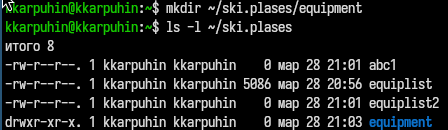
\includegraphics[width=0.7\linewidth,height=\textheight,keepaspectratio]{image/29.png}

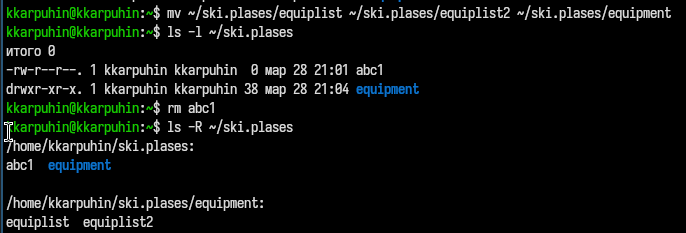
\includegraphics[width=0.7\linewidth,height=\textheight,keepaspectratio]{image/30.png}
\end{frame}

\begin{frame}[fragile]{Создание, перемещение и переименование каталога
\texttt{plans}}
\protect\phantomsection\label{ux441ux43eux437ux434ux430ux43dux438ux435-ux43fux435ux440ux435ux43cux435ux449ux435ux43dux438ux435-ux438-ux43fux435ux440ux435ux438ux43cux435ux43dux43eux432ux430ux43dux438ux435-ux43aux430ux442ux430ux43bux43eux433ux430-plans}
Создал каталог \texttt{\textasciitilde{}/newdir}, переместил его в
\texttt{\textasciitilde{}/ski.plases} и переименовал в \texttt{plans}.

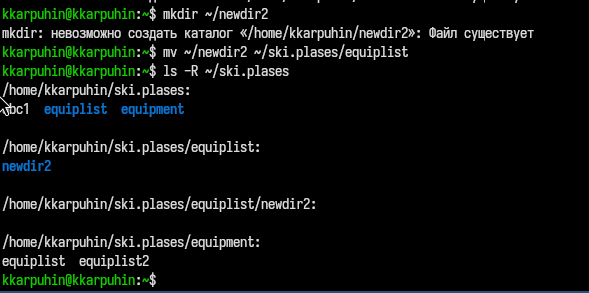
\includegraphics[width=0.7\linewidth,height=\textheight,keepaspectratio]{image/31.png}
\end{frame}

\begin{frame}[fragile]{Изменение прав доступа для файлов}
\protect\phantomsection\label{ux438ux437ux43cux435ux43dux435ux43dux438ux435-ux43fux440ux430ux432-ux434ux43eux441ux442ux443ux43fux430-ux434ux43bux44f-ux444ux430ux439ux43bux43eux432}
Выполнил команды \texttt{chmod} для файлов: -
\texttt{chmod\ 754\ australia} - \texttt{chmod\ 711\ play} -
\texttt{chmod\ 544\ my\_os} - \texttt{chmod\ 664\ feathers}

Результат проверил командой \texttt{ls\ -l}.

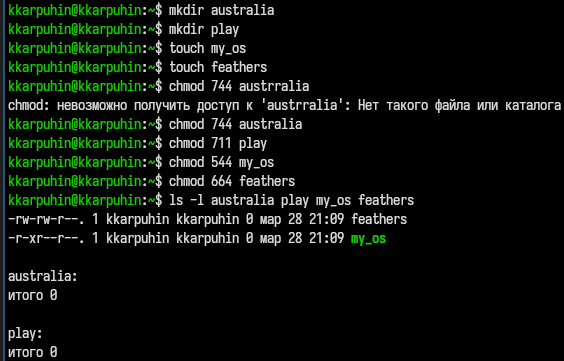
\includegraphics[width=0.7\linewidth,height=\textheight,keepaspectratio]{image/32.png}
\end{frame}

\begin{frame}[fragile]{Упражнение: лишение права на чтение файла
\texttt{feathers}}
\protect\phantomsection\label{ux443ux43fux440ux430ux436ux43dux435ux43dux438ux435-ux43bux438ux448ux435ux43dux438ux435-ux43fux440ux430ux432ux430-ux43dux430-ux447ux442ux435ux43dux438ux435-ux444ux430ux439ux43bux430-feathers}
Лишил владельца права на чтение файла
\texttt{\textasciitilde{}/feathers}
(\texttt{chmod\ u-r\ \textasciitilde{}/feathers}).
\end{frame}

\begin{frame}[fragile]{Попытка просмотра файла \texttt{feathers}}
\protect\phantomsection\label{ux43fux43eux43fux44bux442ux43aux430-ux43fux440ux43eux441ux43cux43eux442ux440ux430-ux444ux430ux439ux43bux430-feathers}
При попытке просмотреть \texttt{\textasciitilde{}/feathers} командой
\texttt{cat} возникла ошибка доступа.

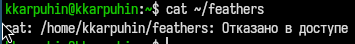
\includegraphics[width=0.7\linewidth,height=\textheight,keepaspectratio]{image/33.png}
\end{frame}

\begin{frame}[fragile]{Попытка копирования файла \texttt{feathers}}
\protect\phantomsection\label{ux43fux43eux43fux44bux442ux43aux430-ux43aux43eux43fux438ux440ux43eux432ux430ux43dux438ux44f-ux444ux430ux439ux43bux430-feathers}
При попытке скопировать \texttt{\textasciitilde{}/feathers} возникла
ошибка доступа.

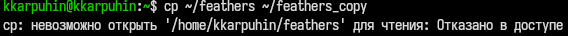
\includegraphics[width=0.7\linewidth,height=\textheight,keepaspectratio]{image/34.png}
\end{frame}

\begin{frame}[fragile]{Возврат права на чтение}
\protect\phantomsection\label{ux432ux43eux437ux432ux440ux430ux442-ux43fux440ux430ux432ux430-ux43dux430-ux447ux442ux435ux43dux438ux435}
Вернул владельцу право на чтение
(\texttt{chmod\ u+r\ \textasciitilde{}/feathers}).
\end{frame}

\begin{frame}[fragile]{Упражнение: лишение права на выполнение каталога
\texttt{play}}
\protect\phantomsection\label{ux443ux43fux440ux430ux436ux43dux435ux43dux438ux435-ux43bux438ux448ux435ux43dux438ux435-ux43fux440ux430ux432ux430-ux43dux430-ux432ux44bux43fux43eux43bux43dux435ux43dux438ux435-ux43aux430ux442ux430ux43bux43eux433ux430-play}
Лишил владельца права на выполнение каталога
\texttt{\textasciitilde{}/play}
(\texttt{chmod\ u-x\ \textasciitilde{}/play}).
\end{frame}

\begin{frame}[fragile]{Попытка перехода в каталог \texttt{play}}
\protect\phantomsection\label{ux43fux43eux43fux44bux442ux43aux430-ux43fux435ux440ux435ux445ux43eux434ux430-ux432-ux43aux430ux442ux430ux43bux43eux433-play}
При попытке перейти в \texttt{\textasciitilde{}/play} командой
\texttt{cd\ \textasciitilde{}/play} возникла ошибка доступа.

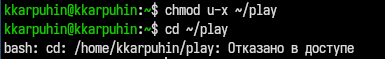
\includegraphics[width=0.7\linewidth,height=\textheight,keepaspectratio]{image/35.png}
\end{frame}

\begin{frame}[fragile]{Возврат права на выполнение}
\protect\phantomsection\label{ux432ux43eux437ux432ux440ux430ux442-ux43fux440ux430ux432ux430-ux43dux430-ux432ux44bux43fux43eux43bux43dux435ux43dux438ux435}
Вернул владельцу право на выполнение каталога
\texttt{\textasciitilde{}/play}
(\texttt{chmod\ u+x\ \textasciitilde{}/play}).
\end{frame}

\begin{frame}[fragile]{Анализ файловой системы: команда \texttt{mount}}
\protect\phantomsection\label{ux430ux43dux430ux43bux438ux437-ux444ux430ux439ux43bux43eux432ux43eux439-ux441ux438ux441ux442ux435ux43cux44b-ux43aux43eux43cux430ux43dux434ux430-mount}
Просмотрел смонтированные файловые системы с помощью \texttt{mount}.


\includegraphics[width=0.7\linewidth,height=\textheight,keepaspectratio]{image/21.png}
\end{frame}

\begin{frame}[fragile]{Анализ файловой системы: файл
\texttt{/etc/fstab}}
\protect\phantomsection\label{ux430ux43dux430ux43bux438ux437-ux444ux430ux439ux43bux43eux432ux43eux439-ux441ux438ux441ux442ux435ux43cux44b-ux444ux430ux439ux43b-etcfstab}
Просмотрел содержимое файла \texttt{/etc/fstab}.


\includegraphics[width=0.7\linewidth,height=\textheight,keepaspectratio]{image/22.png}
\end{frame}

\begin{frame}[fragile]{Анализ файловой системы: команда \texttt{df}}
\protect\phantomsection\label{ux430ux43dux430ux43bux438ux437-ux444ux430ux439ux43bux43eux432ux43eux439-ux441ux438ux441ux442ux435ux43cux44b-ux43aux43eux43cux430ux43dux434ux430-df}
Определил объём свободного пространства командой \texttt{df}.


\includegraphics[width=0.7\linewidth,height=\textheight,keepaspectratio]{image/23.png}
\end{frame}

\begin{frame}[fragile]{Изучение справочных страниц}
\protect\phantomsection\label{ux438ux437ux443ux447ux435ux43dux438ux435-ux441ux43fux440ux430ux432ux43eux447ux43dux44bux445-ux441ux442ux440ux430ux43dux438ux446}
Прочитал \texttt{man} по командам: - \texttt{mount} --- монтирование
файловых систем. - \texttt{fsck} --- проверка и восстановление
целостности файловой системы. - \texttt{mkfs} --- создание файловой
системы на устройстве. - \texttt{kill} --- отправка сигналов процессам.
\end{frame}

\section{Результаты и
анализ}\label{ux440ux435ux437ux443ux43bux44cux442ux430ux442ux44b-ux438-ux430ux43dux430ux43bux438ux437}

\begin{frame}[fragile]{Анализ достигнутых результатов}
\protect\phantomsection\label{ux430ux43dux430ux43bux438ux437-ux434ux43eux441ux442ux438ux433ux43dux443ux442ux44bux445-ux440ux435ux437ux443ux43bux44cux442ux430ux442ux43eux432}
\begin{itemize}[<+->]
\tightlist
\item
  Скопирован и переименован файл \texttt{equipment} →
  \texttt{equiplist}, создан каталог \texttt{ski.plases}, выполнены
  перемещения согласно заданию.
\item
  Настроены права доступа \texttt{754}, \texttt{711}, \texttt{544},
  \texttt{664} для заданных файлов.
\item
  Продемонстрировано влияние прав доступа на возможность чтения и
  выполнения: при отсутствии права на чтение файл нельзя просмотреть или
  скопировать, а без права на выполнение нельзя войти в каталог.
\item
  Изучены смонтированные файловые системы, содержимое
  \texttt{/etc/fstab} и свободное место на дисках.
\item
  Получены краткие характеристики команд \texttt{mount}, \texttt{fsck},
  \texttt{mkfs}, \texttt{kill} из справочной системы.
\end{itemize}
\end{frame}

\begin{frame}[fragile]{Практическая значимость результатов}
\protect\phantomsection\label{ux43fux440ux430ux43aux442ux438ux447ux435ux441ux43aux430ux44f-ux437ux43dux430ux447ux438ux43cux43eux441ux442ux44c-ux440ux435ux437ux443ux43bux44cux442ux430ux442ux43eux432}
\begin{itemize}[<+->]
\tightlist
\item
  Сформированы навыки копирования, перемещения, переименования файлов и
  каталогов в Linux.
\item
  Освоено управление правами доступа с помощью \texttt{chmod}.
\item
  Приобретены умения анализировать состояние файловой системы
  (смонтированные разделы, свободное пространство).
\item
  Расширены знания о системных утилитах для работы с дисками и
  процессами.
\end{itemize}
\end{frame}

\section{Выводы}\label{ux432ux44bux432ux43eux434ux44b}

\begin{frame}[fragile]{Общее заключение}
\protect\phantomsection\label{ux43eux431ux449ux435ux435-ux437ux430ux43aux43bux44eux447ux435ux43dux438ux435}
В ходе лабораторной работы: - Освоены команды для работы с файлами и
каталогами (\texttt{cp}, \texttt{mv}, \texttt{chmod}). - Выполнены
практические задания по копированию, перемещению и переименованию
объектов. - Изучены права доступа и их влияние на операции с файлами и
каталогами. - Получены навыки анализа файловой системы с помощью
\texttt{mount} и \texttt{df}. - Изучены справочные страницы утилит
\texttt{mount}, \texttt{fsck}, \texttt{mkfs}, \texttt{kill}.
\end{frame}

\begin{frame}[fragile]{Выводы}
\protect\phantomsection\label{ux432ux44bux432ux43eux434ux44b-1}
\begin{enumerate}[<+->]
\tightlist
\item
  Команды \texttt{cp}, \texttt{mv}, \texttt{chmod} позволяют гибко
  управлять объектами файловой системы.
\item
  Права доступа играют ключевую роль в безопасности и работоспособности
  системы.
\item
  Утилиты \texttt{mount} и \texttt{df} дают полную картину о
  смонтированных разделах и использовании дискового пространства.
\item
  Справочная система \texttt{man} является незаменимым инструментом для
  изучения новых команд.
\item
  Полученные навыки являются базовыми для дальнейшего освоения
  администрирования Linux.
\end{enumerate}
\end{frame}




\end{document}
